\chapter{Technologies used}

Since we already announced that we are going to work on both Linux and Windows, before diving into the installation process of eBPF on both Linux and Windows, it is important to describe the technologies that allowed us to develop programs using eBPF.

\section{The host environment}

The project started with a single Windows 11 PC serving as the host environment for all research and development activities. 

The computer has a 64 bit operating system with a processor based on x64, a 16 GB RAM and a Solid-State Drive (SSD) with a capacity of 1TB as for storage.
Windows 11, with its user-friendly interface and vast software ecosystem, combined with the power given by the four cores of the Intel Core i7 processor, provided an efficient platform for general computing requirements.

Given the fact that other operating systems were required for this project, the integration of virtualization was crucial to create isolated environments alongside the Windows host.

\section{Virtual machine for Linux development}

For installing and developing programs with eBPF on Linux, a virtual machine running Ubuntu 22.04 was set up within VirtualBox (the version of the Ubuntu operating system is not important).

VirtualBox is a type 2 or hosted hypervisor suitable for individual use and small-scale virtualization scenarios.
It is a software application that runs on top of an existing operating system (called host OS) and provides the capability to create and manage virtual machines. 
Figure \ref{fig:type_2_hypervisor} shows a schematic representation of the architecture just described.
VirtualBox allows you to test, develop and run multiple guest operating systems within your host operating system simultaneously, providing a good level of isolation between the host and guest operating systems.
As a type 2 hypervisor, VirtualBox relies on the host operating system's kernel to manage hardware resources: it uses device drivers and services from the host OS to interact with the physical hardware, which can introduce some overhead and may affect performance compared to a type 1 hypervisor.

\begin{figure}[h]
	\centering
	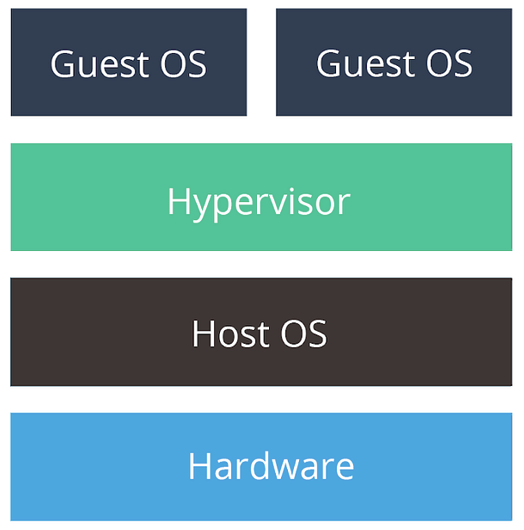
\includegraphics[width=0.7\linewidth]{images/Technologies/type_2_hypervisor.png}
	\caption{Type 2 (or hosted) hypervisor architecture \cite{HypervisorsArchitectures}.}
	\label{fig:type_2_hypervisor}
\end{figure}

Even though VirtalBox relies on the host OS for certain operations, which can lead to performance differences and potential resource conflicts, it was chosen over a type 1 hypervisor for its user-friendly virtualization solution.

The installation process involved creating a virtual disk, configuring memory and CPU allocation and selecting the Ubuntu 22.04 ISO file previously downloaded for installation \cite{UbuntuISOImage}. 
The virtual machine provided a native Linux platform for eBPF program development, compilation and testing.


\section{Virtual machine for Windows development}

Since the main focus is the analysis of eBPF state of art on Windows, the project also demanded the capability to develop eBPF programs specific to the Windows platform. 
For this purpose, the Hyper-V Console Manager, a native Windows feature, was used to create a separate Windows 11 virtual machine.

Hyper-V is a type 1 or bare-metal virtualization software, also known as a Virtual Machine Monitor (VMM), which runs directly on the physical hardware without the need for an underlying host operating system. 
The illustrative representation of the architecture just described is depicted in Figure \ref{fig:type_1_hypervisor}.
As the core software responsible for managing virtual machines and allocating hardware resources to each VM, Hyper-V ensures better security and resource utilization by isolating each VM from others and the host OS. 
With direct access to the physical hardware, it efficiently allocates resources, resulting in improved performance, isolation and scalability compared to type 2 hypervisors like VirtualBox.

\begin{figure}[h]
	\centering
	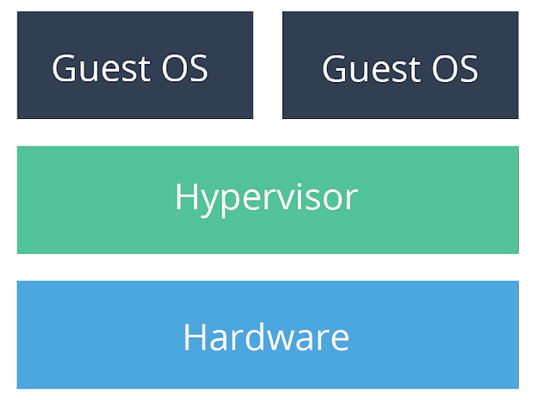
\includegraphics[width=0.7\linewidth]{images/Technologies/type_1_hypervisor.png}
	\caption{Type 1 (or bare metal) hypervisor architecture \cite{HypervisorsArchitectures}.}
	\label{fig:type_1_hypervisor}
\end{figure}

Even though hypervisors are favored for their robustness and scalability, enabling the efficient virtualization of large-scale applications and services, the choice of creating a virtual machine using the Hyper-V Console Manager was dictated by the setup instructions described on the \textit{ebpf-for-windows} GitHub repository \cite{VMSetup}.

We are going to talk about the eBPF installation on Windows later: for now, besides the fact that that he virtual machine was configured with adequate resources to support development tasks effectively, the only thing worth noting is that during the quick creation of the virtual machine the option of ``Windows 11 dev environment'' must be selected (the tutorial tells to choose the ``Windows 10 dev environment'', but Windows 11 works as well).  

The so created isolated Windows 11 development environment provided a controlled space for testing and optimizing eBPF programs on the Windows platform.

\section{Repository of the project}

GitHub is a platform and cloud-based service for software development and collaborative version control using Git, a distributed version control system that tracks changes in any set of computer files, allowing developers to store and manage their code, owned by the company GitHub Inc., whose logo is displayed in Figure \ref{fig:GitHub_logo}.
It provides the distributed version control of Git plus access control, bug tracking, software feature requests, task management, continuous integration and wikis for every project.
It is commonly used to host open source software development projects.

\begin{figure}[h]
	\centering
	
\includegraphics[width=0.7\linewidth]{images/Technologies/GitHub_logo.png}
	\caption{GitHub \textit{Invertocat} logo \cite{GitHubLogo}.}
	\label{fig:GitHub_logo}
\end{figure}

Throughout the course of my master's thesis on eBPF, GitHub was an indispensable platform that played a dual role in enhancing my research journey. 

Firstly, it served as an efficient instrument to share the progress of my work with my  co-advisors and make easier the collaboration during the entire development process. 
Its version control system allowed me to keep track of changes, maintain a detailed history of my project and collaborate consistently with my co-advisors, ensuring a smooth and efficient development workflow. 
By regularly pushing updates to the repository \cite{MasterThesisRepo}, my co-advisors were able to monitor the evolution of my work, review code changes, provide timely feedback and offer valuable suggestions for improvement.

Secondly, GitHub served as an invaluable resource for the eBPF community: during my research, I encountered several repositories (which we will discuss later) dedicated to developing and optimizing eBPF environments, tools and libraries. 
By studying and understanding their implementations, I was able to build upon the expertise and contributions of the open-source community, so that the quality and scope of my research have been enriched.

The open-source spirit of GitHub made knowledge exchange and collective growth easier, enabling me to contribute to the eBPF community while benefiting from the collective expertise it had to offer.
In fact, the public visibility of the GitHub repository of this project opens up the possibility of sharing my work with the wider community. 
By making the repository public, we hope that others can benefit from the knowledge and insights gained during the project, encouraging collaboration and contributions from future researchers and developers in the field of eBPF and its applications.

\todo{CITARE TEXSTUDIO E LATEX}
